% Chapter Template

\chapter{Haskell Type Checking} % Main chapter title

\label{chap:haskell-type-checking}

\graphicspath{{Figures/HaskellTypeChecking}}
In this chapter we delve into the technique overview of type checking Haskell programs. Haskell uses static types, meaning that type checking algorithms are run at time user compiles the code. More specifically, this happens after the parsing is complete (as the complete syntax tree is necessary for type checking), and before any low level code is generated. In a most simplistic sense, type checking returns a binary result: the program is type correct, or it is ill-typed.

\section{Why Haskell}

The main contributions of my thesis are all in the theme of developing systems to improving the programming in Haskell. Despite all the works are developed to be easily extend to other language, there are important reasons why we implemented these tools for Haskell.

\subsection{Haskell In Education}

Being one of the goal of the  Haskell language, teaching programming in undergraduate computer science course is an important application of Haskell.  Many text-books meant for first year computer science courses and introduction to functional programming use Haskell as the learning tool \cite{Bird1998-kv, Davie1992-xv}. Although enthusiasts often argue that Haskell is an ideal platform to teach pure function thinking, the real world university adoption appear to be underwhelming. In fact, help students tackling with the programming errors in Haskell seem to be a common challenge of teaching Haskell \cite{Jun2000-yu, Tirronen2015-nr}. Some suggest teaching Haskell with a reduced feature set to prevent the frustration of complex type errors \cite{Heeren2003-mz}. Our research is hugely motivated by the drive to realize Haskell's educational value as well as the challenges of teaching Haskell in real life.

\subsection{Haskell In Mathematics and Formal Logic}

Another important application for Haskell is its application in discrete mathematics and formal logic. Because its strong type system and enforcement of purely functional computation, Haskell has been stand in the midway of general purpose programming language and a proof assistance. Tools like QuickCheck \cite{Claessen2000-rl} has eased the barrier to write verifiable programs and has since be borrowed to other languages as well. Some proposed using Haskell in hardware verification \cite{Bjesse1998-lh}. However, a common challenge of using these formal systems is its expandability. As larger proof has been constructed by numerous level of abstraction, our confidence in the system and ability to explain are lowered. Our research proposes such interactive explanation system that allow user to check the development of a proof or refutation step by step, each time with a small amount of mental burden. 


\subsection{Haskell's Relatively Small Language Specification}

Although the full language semantics of Haskell was never able to be formally defined \cite{Hudak2007-kn}, it does not stop the language being studied for programming language innovations, nor does it stop researchers making meaningful contributions using this language as platform. Many efforts have made to formalize subsets of Haskell language \cite{FaxEn2002-nd}. Our research in Haskell benefit from the relatively small language specification which allow us to quickly implement new ideas and seek feedback.  We also benefit from the welcoming and vibrant Haskell community to help steer our efforts towards better usability. 




\section{Hindley-Milner Type Inference and Algorithm W}

Type inference, also known as implicit typing is a technique to reduce the number of occurrence of manually ascribing types. Almost all language today employ certain level of type inference. For instance in Java before 10, a common pattern is a user has to declare a variable with a type, often by writing down the class name, and then to initialize the variable, again using the same class name \ref{fig:example-java}. This clearly leads to duplicated knowledge and verbose programs. This has been addressed in later version (Java 10 and later) by using the \texttt{var} keyword \cite{noauthor_undated-an} to declare variables, and the types of the variables can be guessed at compile time based on the right-hand-side of the assignments.  

\begin{figure}[hbt]
  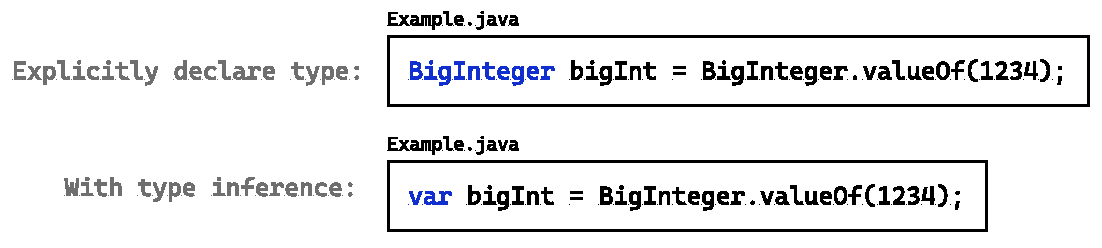
\includegraphics[width=\linewidth]{ExampleJava}
  \caption{
    \label{fig:example-java}
      An example of a typical java program before and after the introduction of \texttt{var} keyword. Before (Top), programmers have to annotate the type, which is identical to the value initializer. After Java 10, this is solved by using the local type inference with the \texttt{var} keyword (Bottom).
    }
\end{figure}

In language like Haskell and ML, not only type inference is applied, its power to detect type error is hugely amplified by the use of the Hindley-Milner type inference. Unlike the example in \ref{fig:example-java} where type inference happens within the assignment statement, meaning that the compiler will complain if it cannot gather enough information about the type when analyzing this line, with HM-based type inference, the compiler will delay making any assertions, and continue type-checking the rest of the program. 

The Hindley-Milner Type System \cite{Damas1982-zw} is foundational parts of type inference in many functional programming languages, including ML, Haskell, and Elm. The Hindley-Milner Type System, named after its inventors Roger Hindley and Robin Milner, is a type system that can automatically infer the types of expressions in a language with no annotations required. The system provides polymorphic typing, meaning that a variable can be assigned multiple different types automatically based on its usage context, making it easier to write flexible, reusable code without compromising type safety. In many languages that uses this system, it is proven that every expression will be assigned a most general type (principal type) based on its usage. 



\begin{figure}[hbt]
    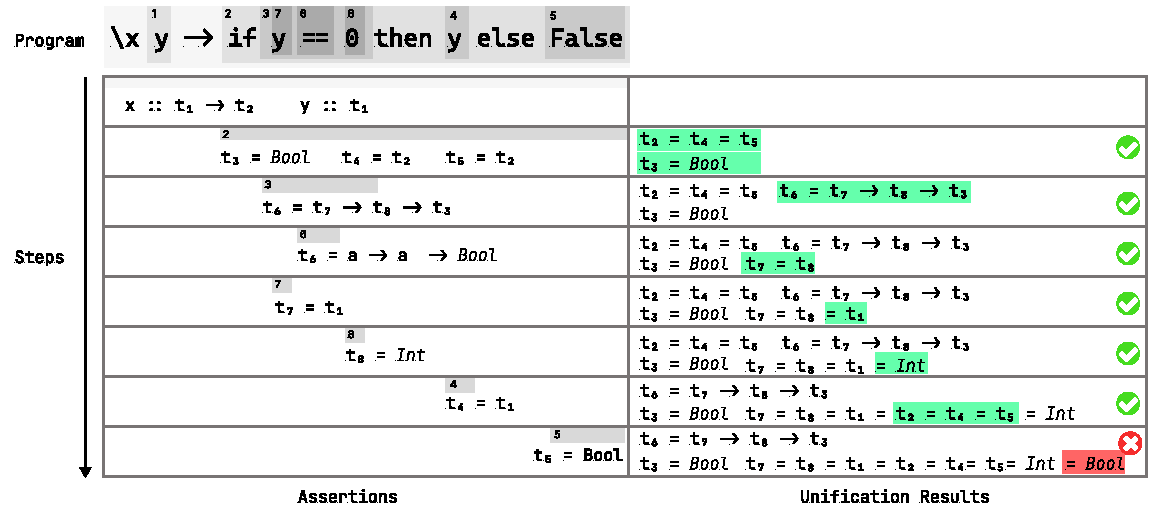
\includegraphics[width=\linewidth]{Hindley-Milner}
    \caption{
      \label{fig:hindley-milner}
        An illustration of Hindley Milner Type Checking}
\end{figure}


\textbf{Algorithm W} The original version of Hindley-Milner type system uses an algorithm -- W -- to identify the most general types for every expression. Algorithm W scans the whole program and produce the most generous types for each expression. The algorithm works by first assuming that each expression has a unique type variable associated with it,  it recursively inspects into the substructure of the program, and collecting constraints and apply unification \ref{fig:hindley-milner}. Depend on the type of syntax node, during a step new variables may be created, variables may unify with other variables or concrete types. If at anytime the unification step fails, the type-checking stops, and the location from which the last constraint is generated will be reported as type error.


Despite the seismic influence in type theory, and the conciseness of programming style it helps achieved,  Hindley-Milner type system introduced some setbacks in terms of usability. More specifically, its error message when unable to complete the process of type inference leads to a lot of confusions to the users. 

Because of the way unification is carried out, only one constraint (the last one added) is reported in the type error and the other end of conflict is unable to be retrieved. Unlike in the Java example where programmers only needs to scan the source code for one line, with Hindley-Milner-based type system, the potential root cause may lie at anywhere in the source code.

\textbf{Algorithm M} 
Others proposed similar algorithm M \cite{Lee1998-fx}, which instead of carry out type inference bottom up, it carries the outer constraints into the inner structure, achieving a top-down type inference, and better error messages in some cases. 

\begin{figure}[hbt]
  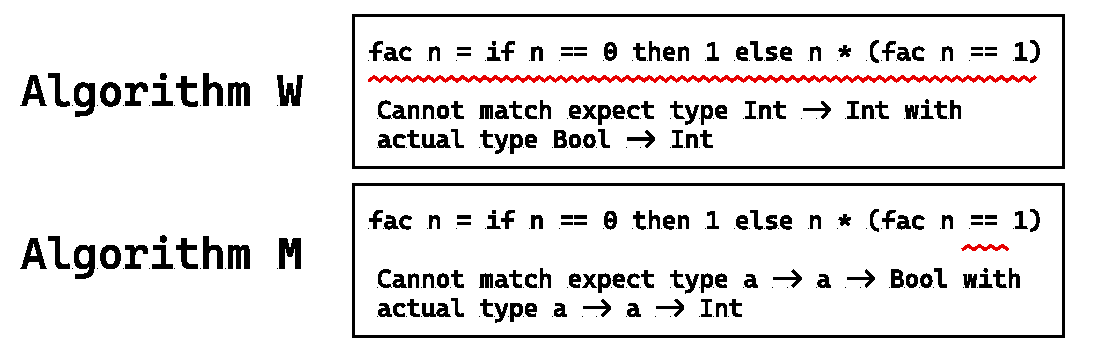
\includegraphics[width=0.8\linewidth]{AlgorithmWM1.pdf}
  \caption{
    \label{fig:algorithm-m-1}
      An example where Algorithm M out-guessed Algorithm W, reporting a more plausible error location.}
\end{figure}


\begin{figure}[hbt]
  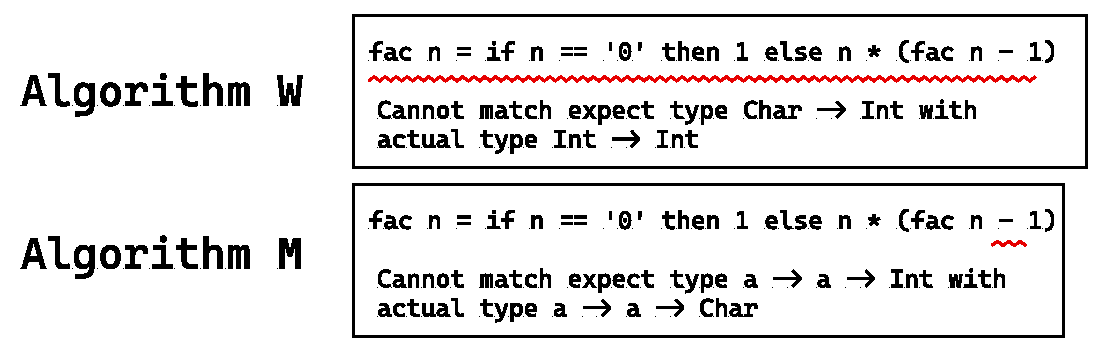
\includegraphics[width=0.8\linewidth]{AlgorithmWM2}
  \caption{
    \label{fig:algorithm-m-2}
    An example where Algorithm M may miss the correct location. It is more plausible here \texttt{'0'} is a typo.}
\end{figure}


As a result, algorithm M is able to identify certain errors more accurately than algorithm W \ref{fig:algorithm-m-1}. However, it is equally misleading in some other cases \ref{fig:algorithm-m-2}. An important lesson can be learned from these different approach of type inference is that there is no method that will ensure the result will match programmers' true intention with the code. At the core, algorithm M and algorithm W suffer from the same issue: the unification is done one step at a time, and the earlier constraints are lost once they are successfully unified. And rather than ambitiously pinpoint the place where the root cause lies, a more realistic goal might be to succinctly representing type error without making assumption.



\section{Type Error Slicing}

Type error slicing \cite{Tip2001-qn, Haack2004-fr} is a technique aim to represent type error by including more useful information to programmer. Compared to the Hindley-Milner approach, it relies on delay the unification until all constraints are generated. Two important ideas have been employed in type error slicing: 


\begin{enumerate}
  \item {
    Labeled constraints. Assign constraints to locations in programs, and these locations are later on retrieved, and identified as part of the error diagnosis. 
  }
  \item {
    Minimal unsatisfiability analysis. Finding the minimal unsatisfiable locations that contributed to a type error  as a standard process of type error diagnosis. In practice minimal unsatisfiable locations avoid being too general as in algorithm W, and avoids being too biased as in both algorithm W and algorithm M. 
  }
\end{enumerate}


\begin{figure}[hbt]
  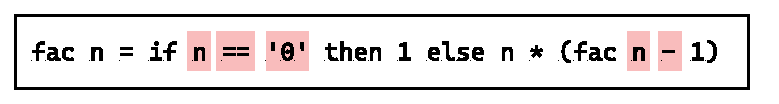
\includegraphics[width=0.5\linewidth]{TypeErrorSlicing.pdf}
  \caption{
    \label{fig:type-error-slicing}
      An example of type error slicing}
\end{figure}

Compared to traditional tools, type error slicing show complete error locations \ref{fig:type-error-slicing} and programmers are able to reason about the type error because both sides of the typing conflict is included. 

Over the years, type error slicing has become the go-to approach for optimizing type errors. The method of producing minimal unsatisfiable locations have been improved and generalized by many. In general, the process involves removing constraints one at a time and checking the feasibility of the system changes. Different underlying constraint languages have been studied to encode more advanced type system features. This includes using SMT \cite{Pavlinovic2015-ke}, Constraint Handling Rules \cite{Stuckey2003-pz}, and so on. 



\section{Interactive Type Debugging}

In conventional program slicing approaches, a Minimal Unsatisfiable Subset (MUS) is typically used to represent a single type error, thereby providing locations for the type error report. However, we have identified two significant limitations inherent in MUS-based localization and diagnosis:


\begin{figure}[hbt]
  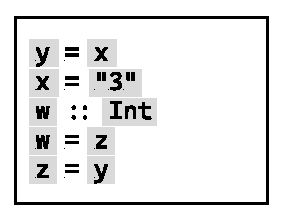
\includegraphics[width=0.5\linewidth]{SlicingCounterExample}
  \caption{
    \label{fig:slicing-counter-example}
      An example where type error slicing essentially highlight every location in the program.}
\end{figure}

MUS-based error slicing can effectively eliminate program locations that are not contributing to a type error. However, research indicates that program slicing can effectively reduce only around 30\% of the code size that is required to understand a type error \cite{binkley_empirical_2007}. Further reduction is challenging with the knowledge of MUS alone due to the MUS's minimality. For instance, in the code shown in \ref{fig:slicing-counter-example}, type error slicing essentially highlight every location in the program. Clearly, there are more important information needs to be encoded in the type error.

Chameleon \cite{Stuckey2003-pz} is a project that was created as a command-line tool that in the early 2000s to improve type error reporting 
for the Haskell programming language. Similar to other type error slicing approach, Chameleon used a more general constraint language -- CHR -- which in turn allow more flexible constraints relations can be defined in the constraint language. This is signified by the successful support of advanced type-level features such as type class and functional dependencies. More importantly, Chameleon employed the notion of interactive type debugging. In the example, Chameleon not only highlighted all the relevant locations, it also reflects the fact that two sets of potential types (most general unifiers) can be found in the ill-typed program, and they can be trace back to two sets of locations in the source code. Programmers can proceed to query the type information of either potential resolution as if the type error has been resolved.


\begin{figure}[hbt]
  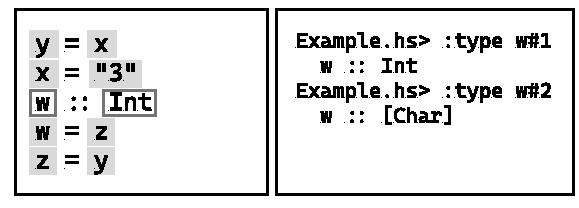
\includegraphics[width=0.8\linewidth]{ChameleonInteractive}
  \caption{
    \label{fig:chameleon-interactive}
      An example where type error slicing essentially highlight every location in the program.}
\end{figure}

\section{The Analysis Of An Unsatisfiable System}

One advantage of using a constraint based type system is that it offers many tools to understand the unsatisfiability of a system. In terms of programming language, the most useful tool we use is Minimal Unsatisfiable Subset (MUS).  MUS detection aims to find the smallest subset of constraints that still renders the system infeasible. For an ill-typed program, this means finding a minimal set of locations that contain a type error. Although finding such a subset can be computationally expensive, it is useful because it represents the type error in more than one location, and contains two sides of the conflict. This is often necessary knowledge in understanding any kinds of conflicts.


Other than MUS, minimal correction set (MCS) and  maximal satisfiable subset (MSS) are useful subsets of the constraint system as well. We give the formal definition of these subsets and their type theoretic interpretation.


[More examples from the prev section]


– A minimal unsatisfiable subset (MUS) $M$ of a constraint system $C$ is a subset $M \subseteq C$ such that $M$ is unsatisfiable and $ \forall{c} \in M : M \setminus \{c\}$ is satisfiable. An MUS can be seen as a minimal explanation of the infeasibility of the constraint system. MUSes have been used extensively, mostly in combination with programming slicing, as a means to explain type errors. An MUS of type system constraints encode a path of reasoning connecting all evidence from one location of the conflict to another.


– A minimal correction set (MCS) $M$ of a constraint system $C$ is a subset $M \subseteq C$ such that $C \setminus M$ is satisfiable and $\forall{S} \subset M : C \setminus S$ is unsatisfiable. MCSes are so named because their removal from $C$ can be seen to “correct” the infeasibility. In an ill-typed program, an MCS can be seen as the ``cause" of a type error; removing any MCS will result in the system being well-typed. Goanna uses an MCS to represent potential causes of a type error. Each MCS contains the set of locations that need to be changed to fully resolve the type error.

  

– A maximal satisfiable subset (MSS) $M$ of a constraint system $C$ is a subset $M \subseteq C$ such that M is satisfiable and $\forall{c}\ in\ C \setminus M:M\cup\{c\}$ is unsatisfiable. The definition of an MSS is symmetric to that of a MUS, with `satisfiable' and `unsatisfiable' swapped along with maximal for minimal. MCS and MSS are complement sets of each other. In an ill-typed program, an MSS can be seen as the resulting typing environment if a type error is fixed by relaxing the MCS.

\subsection{MUS Enumeration}
One observation we can make about the  Minimal Unsatisfiable Subsets is that it is often not unique. It is possible for an unfeasible system to contain a finite number of MUS’s. In practice, existence of multiple MUSes indicates that there are multiple sources of conflict. Enumerating multiple MUS/MCS in this case may provide better insights over the root cause and how to address them properly


However, the problem of MUS enumeration is that it is very computationally expensive. In the most naive approach, it requires exploring the power set of all constraints in the constraint system. In fact, most of the effective enumeration algorithms today rely on heuristics, and they provide performance improvements on a case-by-case basis. MARCO~\cite{Liffiton2016-xi} and MUST~\cite{Bendik2020-pz} are examples of such an approach. They use heuristics to avoid traversing a large chunk of the subsets each representing a permutation of which constraints to be relaxed and which not.


\begin{figure}[hbt]
  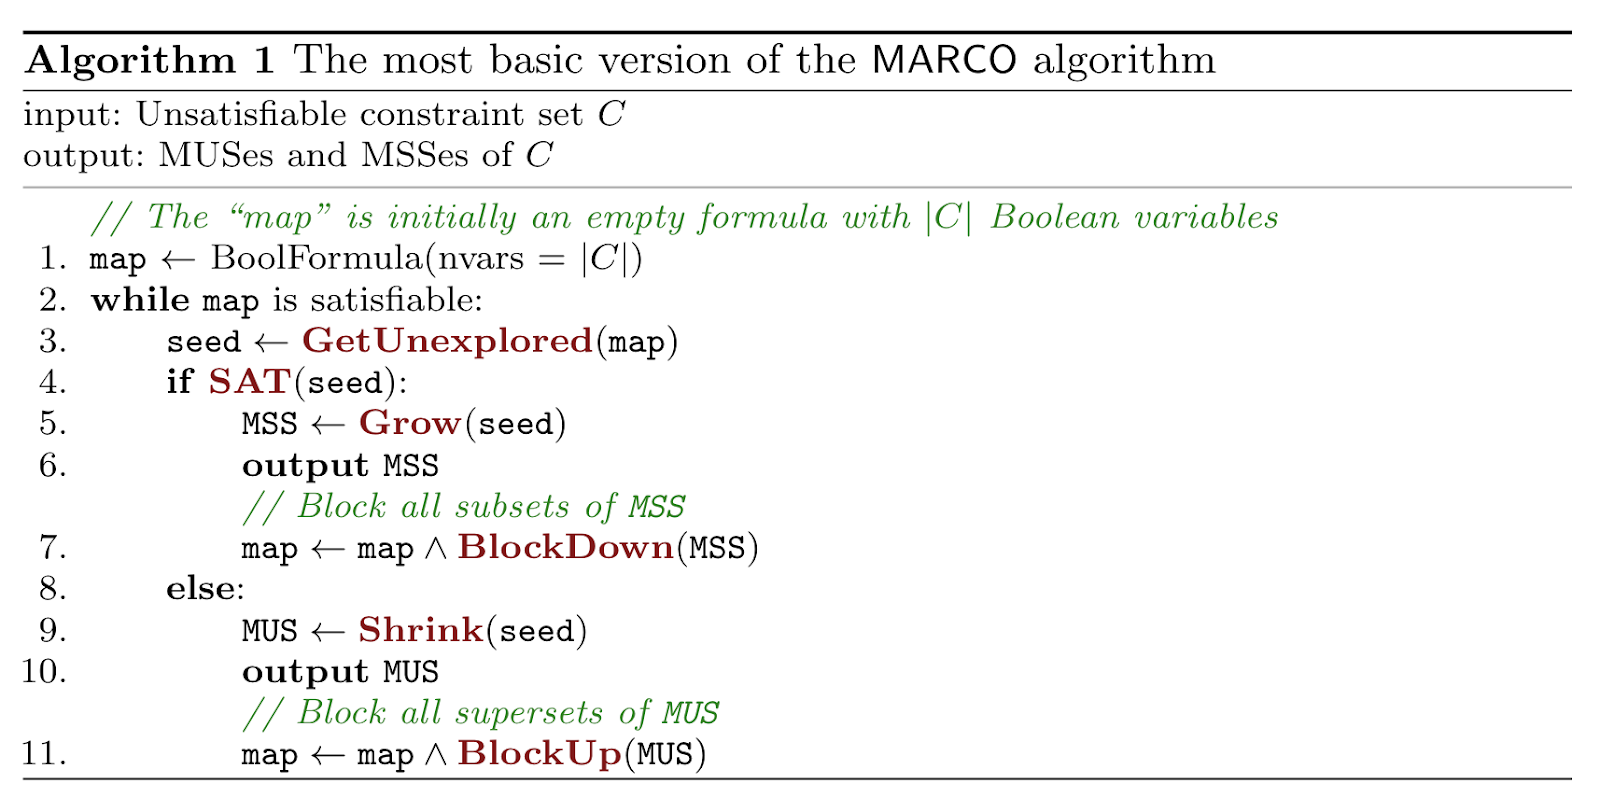
\includegraphics[width=\linewidth]{MarcoAlgo}
  \caption{An simple implementation of the MARCO algorithm}
\end{figure}


\begin{figure}[hbt]
  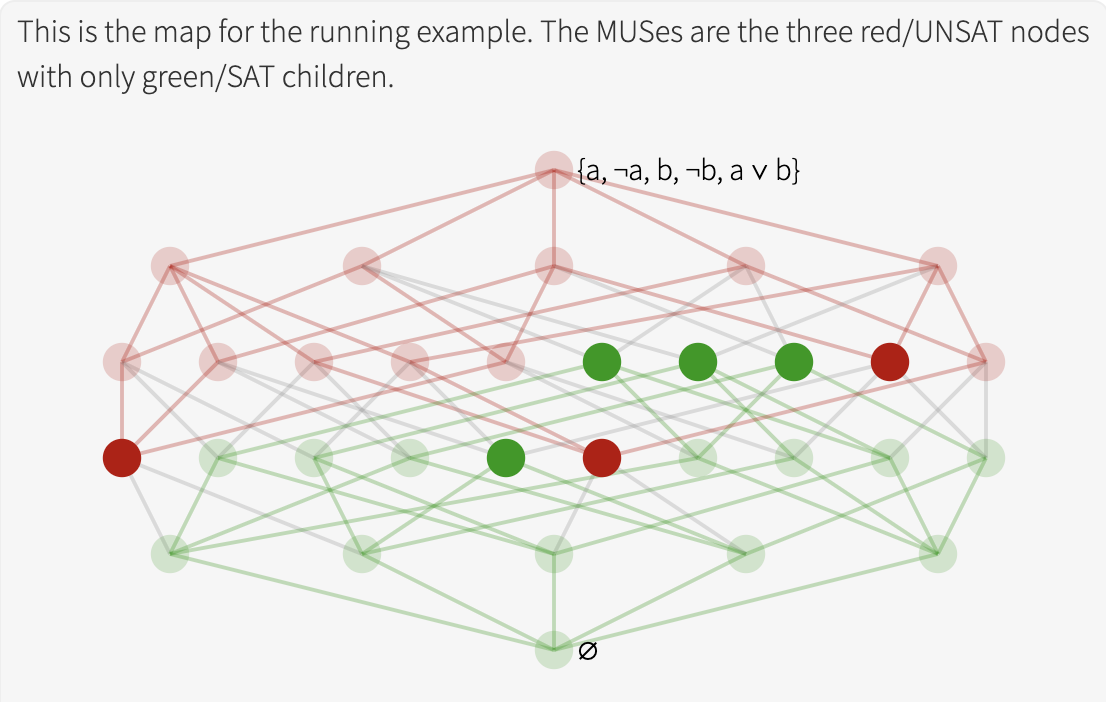
\includegraphics[width=\linewidth]{MarcoViz}
  \caption{An illustration of how MARCO finds all MUSes}
\end{figure}
  

\section{Three Classes of Type Error}

I propose a useful categorization of type errors. This categorization allows a formal study of the tools that is necessary to cover the information of a given type error.  Because we have covered MUS and MUS enumeration, it is now possible to discuss 3 categories of type error based on the feasibility of representing them in a single MUS.

\subsection{Multi-step Type Error}
\begin{figure}[hbt]
  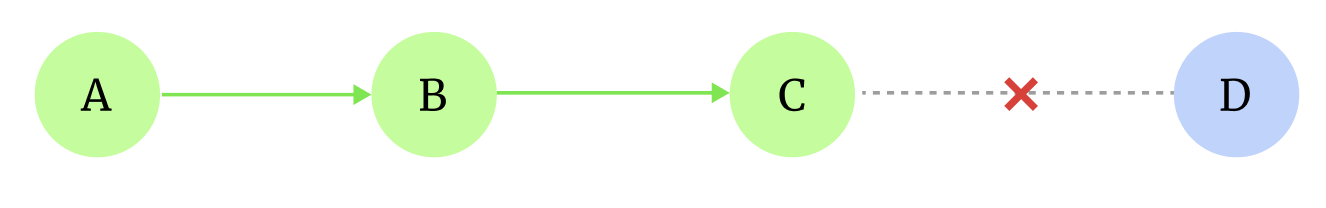
\includegraphics[width=0.5\linewidth]{Multi-step}
  \caption{}
\end{figure}

Multiple-step type errors contain a chain of reasoning steps, or a series of attempts to unify two logical terms. There is no possible way to successfully complete all the unification. However, removing any one of the unification steps will make all other steps feasible. In the error presented in the above figure, the error can be represented in a single MUS {A, B, C, D}.

\subsection{Multi-witness Type Error}
\begin{figure}[hbt]
  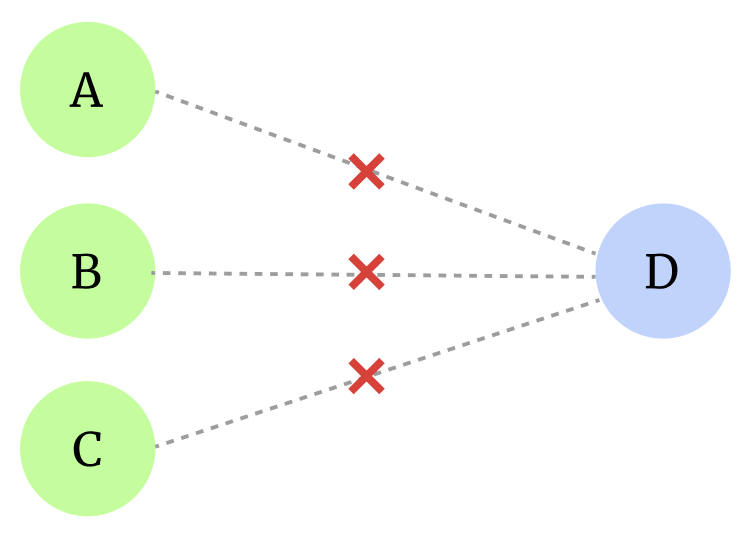
\includegraphics[width=0.5\linewidth]{Multi-witness}
  \caption{}
\end{figure}
A Multiple-witness type error occurs when one side of the conflict contains multiple locations (witnesses) suggesting the same typing assignment. Removing one such location, the type error will remain. In the example, there are three MUSes: {A, D}, {B, D}, {C, D}. Therefore, this type of error cannot be succinctly represented by a single MUS.

\subsection{Multi-party Type Error}
\begin{figure}[hbt]
  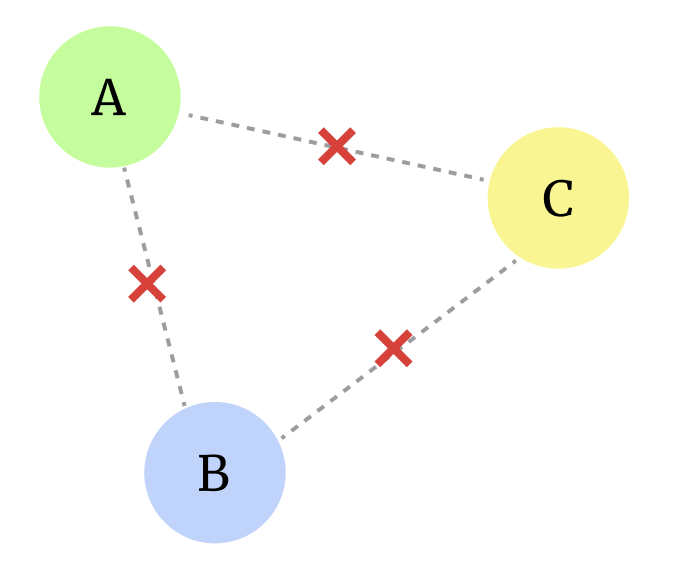
\includegraphics[width=0.5\linewidth]{Multi-party}
  \caption{}
\end{figure}

A Multiple-party type error is an error where multiple type irreconcilable assignments can be obtained from locations of the source code. In the provided example, there are 3 MUS: {A, B}, {A,C}, {B,C}. Therefore, this type of error cannot be succinctly represented by a single MUS.

\begin{figure}[hbt]
  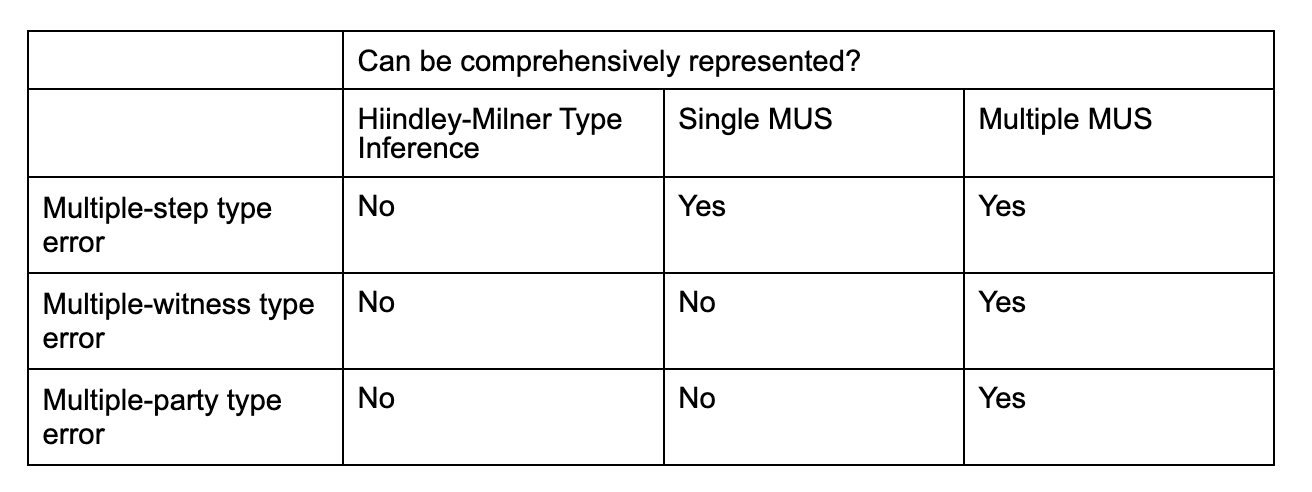
\includegraphics[width=\linewidth]{Compare}
  \caption{}
\end{figure}

\section{Conclusion}
In this chapter, we established a subset of the Haskell language by defining its syntax, and typing rules. We explored two avenues to type-check a program in such language and obtain principle types: using the Hindley-Milner type system and using constraint-based type system. In addition, we explored some type error analysis tools that are enabled by using a constraint based type system, and how these tools are applied to three different kinds of type errors. We will explore them in the next two chapters.
